\providecommand{\main}{..}
\documentclass[\main/main.tex]{subfiles}

\begin{document}
    \justify
    \subsection{Badanie wpływu wartości wag początkowych na szybkość uczenia perceptronu prostego}
    \paragraph{}
    Badanie ma na celu (???) wpływu wartości wag początkowych na działanie perceptronu prostego. Badania przeprowadzone zostały dla unipolarnej funkcji aktywacji oraz unipolarnego zbioru uczącego. Wykorzystano współczynnik uczenia a = 0.05.
    
    \paragraph{}
    Zbadano natomiast następujące przedziały:
    \begin{itemize}
     \item (-1, 1)
     \item (-0.8,  0.8)
     \item (-0.6, 0.6)
     \item (-0.4, 0.4)
     \item (-0.2, 0.2)
     \item (-0.05, 0.05)
     \item (0, 0)
    \end{itemize}
    
    \paragraph{}
    Tak jak zostało to wcześniej wspomniane, prezentowane wyniki są wartościami uśrednionymi, \\hline
    uzyskanymi w skutek wielokrotnego uruchomienia algorytmu i prezentują się one następująco.

    \begin{figure}[H]
    \centering
    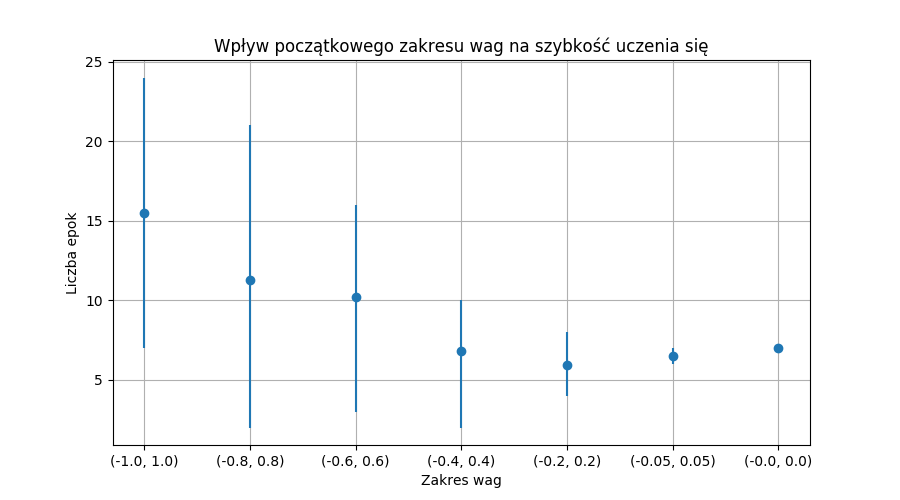
\includegraphics[scale=0.6]{test_weights_SimplePerceptron_10}
    \caption{Wyniki badań uzyskane w skutek 10 uruchomień}
    \end{figure}

    \begin{figure}[H]
    \centering
    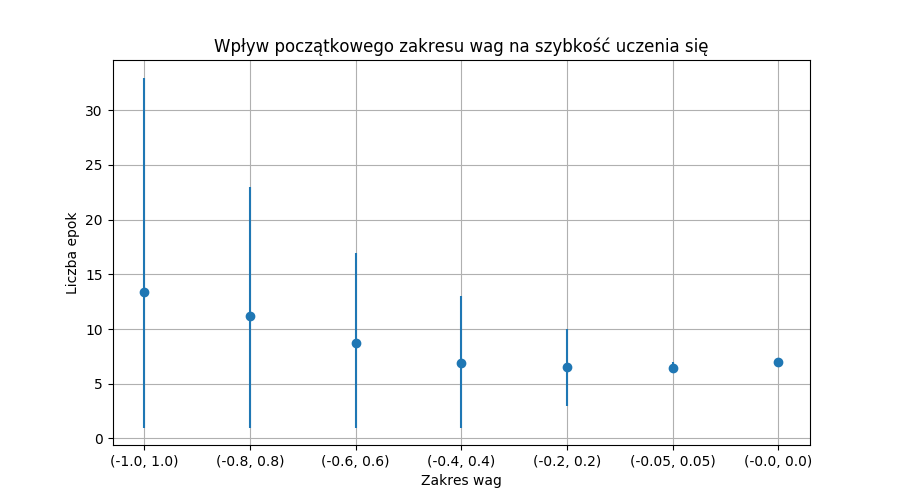
\includegraphics[scale=0.6]{test_weights_SimplePerceptron_100}
    \caption{Wyniki badań uzyskane w skutek 100 uruchomień}
    \end{figure}
    
    \paragraph{}
    W przeprowadzonych badaniach można zauważyć wzrost liczby epok wymaganych do dobrania odpowiednich wag, wraz ze wzrostem wielkości przedziału losowanych wag. Wynika to z faktu, że w przypadku dużych przedziałów wag mogą one wylosować skrajnie różne wartości. Duża różnica między początkową, a optymalną wartością wagi prowadzi, przy stałym współczynniku uczenia, do wzrostu wymaganej liczby epok, a co za tym idzie czasu wymaganego na ukończenie treningu. Wraz ze spadkiem wymaganej liczby epok, zmniejsza się także rozmiar przedziału nieufności, oznacza to, że w przypadku małego przedziału wag wyniki są bardziej zróznoważone i powtarzalne.

    \justify
    \subsection{Badanie wpływu współczynnika uczenia  na szybkość uczenia perceptronu prostego}
    \paragraph{}
    Badanie ma na celu (???) wpływu wartości współczynnika uczenia na działanie perceptronu prostego. Badania przeprowadzone zostały dla unipolarnej funkcji aktywacji oraz unipolarnego zbioru uczącego. Przedział wag do badania został wybrany na podstawie poprzednich obserwacji i ma wartość [-0.2, 0.2].
    
    \paragraph{}
    Badania przeprowadzono na następujących wartościach współczynnika.
    \begin{itemize}
    \item 0.01
    \item 0.05
    \item 0.1
    \item 0.2
    \item 0.5
    \item 0.8
    \item 1.0
    \end{itemize}
    
    Wynikiem przeprowadzonych badań są następujące wykresy:
    
    \begin{figure}[H]
    \centering
    \begin{subfigure}{.5\textwidth}
    \centering
    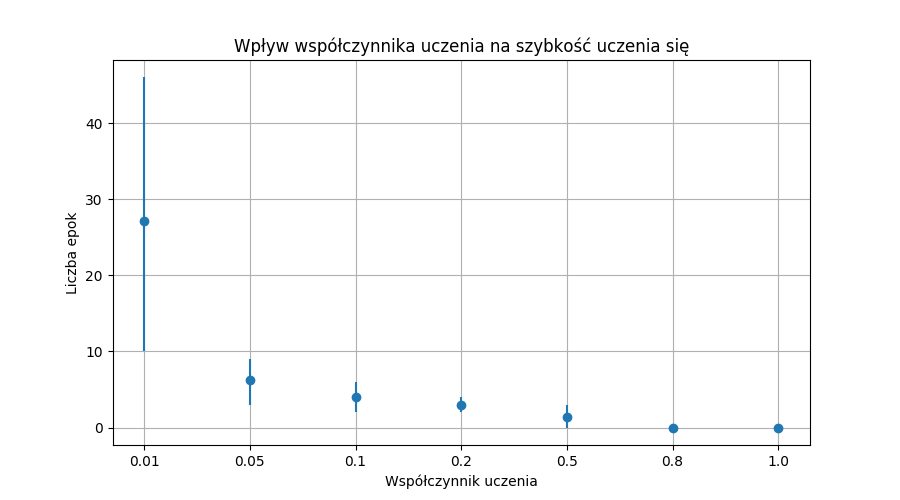
\includegraphics[width=1.1\linewidth]{test_LR_SimplePerceptron_100_epochs}
    \caption{Liczba epok w zależności od współczynnika uczenia}
    \label{fig:lr_sp_epochs}
    \end{subfigure}%
    \begin{subfigure}{.5\textwidth}
    \centering
    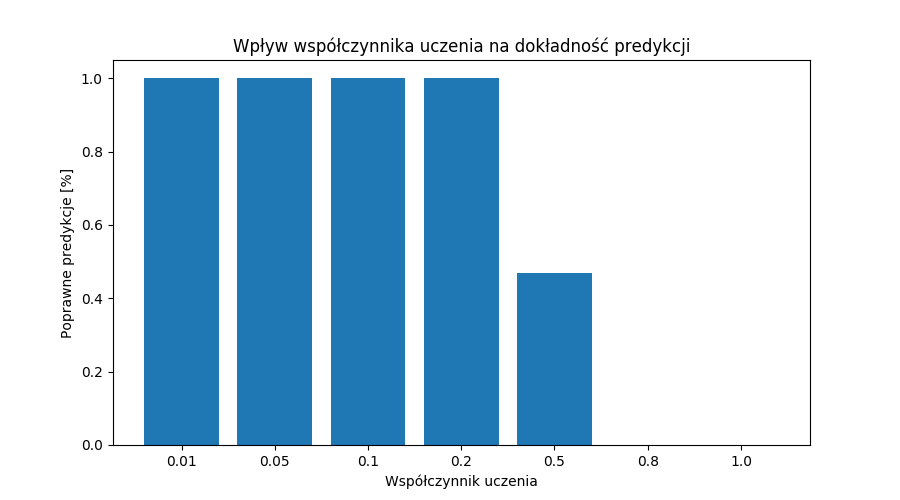
\includegraphics[width=1.1\linewidth]{test_LR_SimplePerceptron_100_correctness}
    \caption{Procent prawidłowych predykcji w zależności od współczynnika uczenia}
    \label{fig:lr_sp_correctness}
    \end{subfigure}
    \caption{Wpływ współczynnika uczenia na szybkość i jakość treningu}
    \label{fig:test}
    \end{figure}
    
    \paragraph{}
    Na pierwszy rzut oka widoczny jest spadek wymaganej liczby epok wraz ze wzrostem współczynnika uczenia. Jednak obserwacja ta nie jest całkowicie poprawna, ze względu na to, że współczynnik uczenia o wartości większej niż 0.5, uniemożliwiał perceptronowi odnalezenie odpowiednich wag. Co widoczne jest na drugim wykresie przedstawiającym procent poprawnych predykcji. Dodatkowo wraz ze wzrostem współczynnika uczenia można zauważyć zmniejszanie się przedziału nieufności. Dla współczynnika o wartości \textbf{0.01} występowały duże wahania pomiędzy kolejnymi testami. Najlepsze wyniki uzyskały współczynnik o wartości \textbf{0.2}, który otrzymał bezbłędny wyniki przy najmniejszej liczbie epok, dodatkowo mały przedział nieufności wskazuje na to, że podobne wyniki otrzymane zostały w każdym z stu uruchomień algorytmu. Podsumowując, zbyt mały współczynnik uczenia wydłuża czas potrzebny na przeprowadzenie treningu dodatkowo powodując dużą różnorodność w liczbie epok między kolejnymi uruchomieniami algorytmu. Zbyt duży współczynnik natomiast całkowicie uniemożliwia przeprowadzenie udanego treningu.
    
    \subsection{Badanie wpływu funkcji aktywacji na szybkość uczenia perceptronu prostego}
    Decyzję o aktywacji neuronu można przeprowadzić na podstawie wielu funkcji. Badanie skupiło się na zaobserwowaniu zmian w czasie trwania treningu przy różnych funkcjach aktywacji. W przeprowadzonych badaniach wykorzystano współczynnik uczenia równy 0.1 oraz początkowy przedział wag wynoszący [-0.2, 0.2].
    
    \paragraph{}
    Badania przeprowadzono na następujących funkcjach aktywacji:
    \begin{itemize}
     \item Funkcja bipolarna
     \item Funkcja unipolarna
    \end{itemize}
    
    Po przeprowadzeniu pomiarów otrzymano następujące wyniki:
    
    \begin{figure}[H]
    \centering
    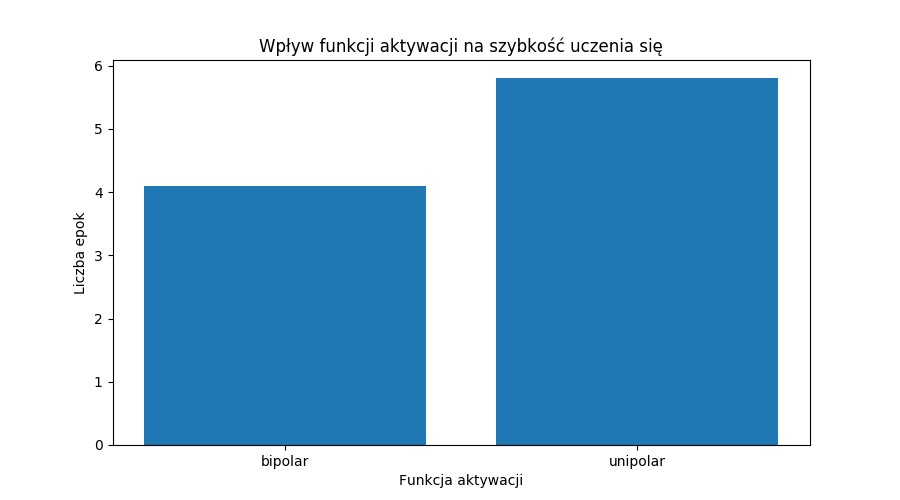
\includegraphics[scale=0.6]{test_activation_SimplePerceptron_10}
    \caption{Wyniki badań uzyskane w skutek 10 uruchomień}
    \end{figure}

    \begin{figure}[H]
    \centering
    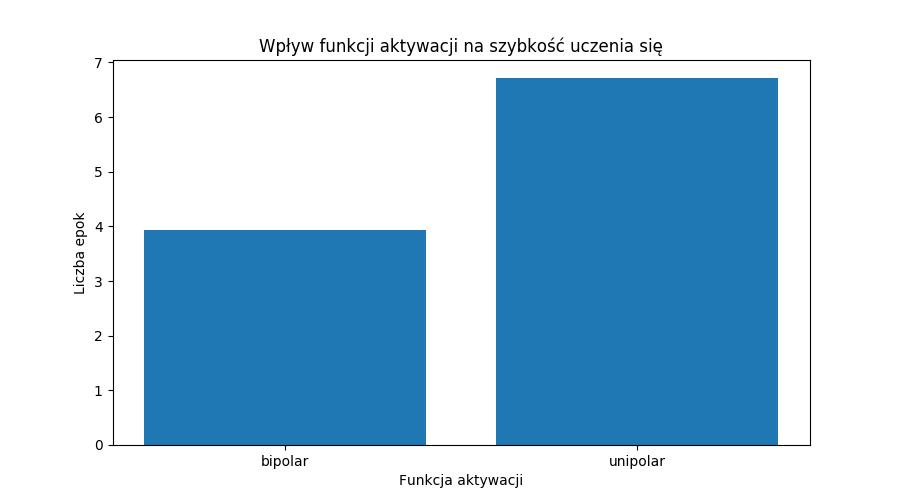
\includegraphics[scale=0.6]{test_activation_SimplePerceptron_100}
    \caption{Wyniki badań uzyskane w skutek 100 uruchomień}
    \end{figure}
    
    \paragraph{}
    \justify
    Jak można zauważyć funkcja bipolarna uzyskuje znacznie lepsze wyniki niż funkcja unipolarna. Wpływ na otrzymane wyniki ma jednak to, że w obu przypadkach użyto tej samej wartości współczynnika uczenia. W przypadku funkcji unipolarnej błąd, który używany jest do poprawienia wag może przyjąć wartości ze zbioru [-1, 0, 1]. Jednak użycie funkcji bipolarnej powoduje, że zbiór możliwych błędów ma postać [-2, 0, 2]. Wagi aktualizowane są więc o większe wartości, co umożliwia szybsze dobranie optymalnych wag.
    
\end{document}
